\def\year{2017}
%File: formatting-instruction.tex
\documentclass[letterpaper]{article}
\usepackage{aaai}
\usepackage{times}
\usepackage{helvet}
\usepackage{courier}
\usepackage{subfigure}
\usepackage{algorithm}
\usepackage{multirow}
\usepackage{multicol}
\usepackage{algpseudocode} %format of the algorithm
\usepackage{color}
\usepackage{url}
\usepackage{latexsym}
\usepackage{graphicx}
\usepackage{epstopdf}
\usepackage{epsfig}
\usepackage{amsmath, bm}
\usepackage{amsfonts}
\usepackage{enumitem}
\usepackage{ulem}
\normalem
\frenchspacing
\setlength{\pdfpagewidth}{8.5in}
\setlength{\pdfpageheight}{11in}
\pdfinfo{
/Title (Insert Your Title Here)
/Author (Put All Your Authors Here, Separated by Commas)}
\setcounter{secnumdepth}{0}  
 \begin{document}
% The file aaai.sty is the style file for AAAI Press 
% proceedings, working notes, and technical reports.
%
\title{PKUICST at TREC 2017 Real-Time Summarization Track:\\
Push Notifications and Email Digest
}
\author{Jizhi Tang \quad Chao Lv \quad Lili Yao \quad Dongyan Zhao\footnote{Corresponding author} \\
\{tangjizhi, lvchao, yaolili, zhaody\}@pku.edu.cn\\
\\
Institute of Computer Science and Technology\\
Peking University, Beijing 100871, China\\
}

\maketitle
\begin{abstract}
\begin{quote}
In this paper, we describe our approaches and corresponding results in the Real-Time Summarization(RTS) track at the 2017 Text Retrieval Conference(TREC).
The main idea is to build a two-stage filter system for both scenario A and B. 
In the first stage, tweets are filtered according to its relevance score to a particular topic,
while in the second stage, they are filtered according to its novelty score to previous submitted tweets.
We tried several approaches to model the text similarity, such as negative KL-divergence and cosine distance, as well as blending models.
Especially, in scenario A, the push notification scenario, we designed a decoupled system that can maintain high availability in order to meet the real-time requirements. 
The experiment results show that our methods reach good performance with respect to several metrics such as EG-p and nDCG-p.
\end{quote}
\end{abstract}

\section{Introduction}
Microblog, such as Twitter and Weibo, has become one of the most important accesses for people to get information.
However, finding out helpful information from massive microblogs by hand can be very difficult and exhausting.
Building an automatic system that helps to pick out specific microblog is a good solution.
The TREC 2017 Real-Time Summarization (RTS) Track aims to explore techniques that helps build such systems.
There are two scenarios contained in the RTS Track: 

\begin{itemize}
\item \textbf{Scenario A (push notification):}
Content that is identified as relevant and novel by a system based
on the user's interest profile should be sent to the user in a timely fashion. 
\item \textbf{Scenario B (email digest):}
Participating systems should identify tweets and aggregate them into an email digest.
The email should be periodically sent to a user. Under that circumstances,
users can read a longer story about the contents.
\end{itemize}

For both scenario A and B, we perform a two-stage filter system separately.

In push notification scenario, our system contains three function modules, Filter Module, Judge Module and Submit Module, and two tables, i.e. Pre-process Table and Submit Table, that transfer data between modules. The Filter Module listens to the tweet sample stream, roughly filter out tweets that obviously     irrelevant to the interest profiles, and insert the remain tweets into the Pre-process Table. The Judge Module continuously detects new tweets from the Pre-process Table, and compute the relevance score between those tweets and the interest profiles. A tuned relevance threshold $\alpha$ is utilized to judge whether a specific tweet and an interest profile are relevant. Then, for every relevant profile, we compute   the novelty score between current tweet and previous submitted tweets. Similarly, a novelty threshold $\beta$ is used to determine whether a tweet is novel. Those tweets passed the two threshold will be inserted to the Submit Table. Finally, the Submit Module submit tweets in the Submit Table to the Evaluation Broker. The independence of the three module guarantees that the system can recover quickly and safely from system crash.

In email digest scenario, we directly precess the tweets from Pre-process Table. The whole procedure is basically the same as Judge Model in scenario A. Two threshold are performed to filter out those 'relevant but novel' tweets. the only difference is that after the filtering, we sort the tweets by the relevance score for every interest profile, and select the top 100 tweets per interest profile per day. 


\section{Method}

In this section, we discuss our system design thoroughly. Fig.\ref{fig:system} shows the architecture of our system. The Pre-process Module and the Pre-process Table are actually shared by both scenario A and B, we take these together as an independent part, Preliminaries. And then Scenario A and B will be discussed separately.  

\begin{figure*}[htbp]
\centering {
	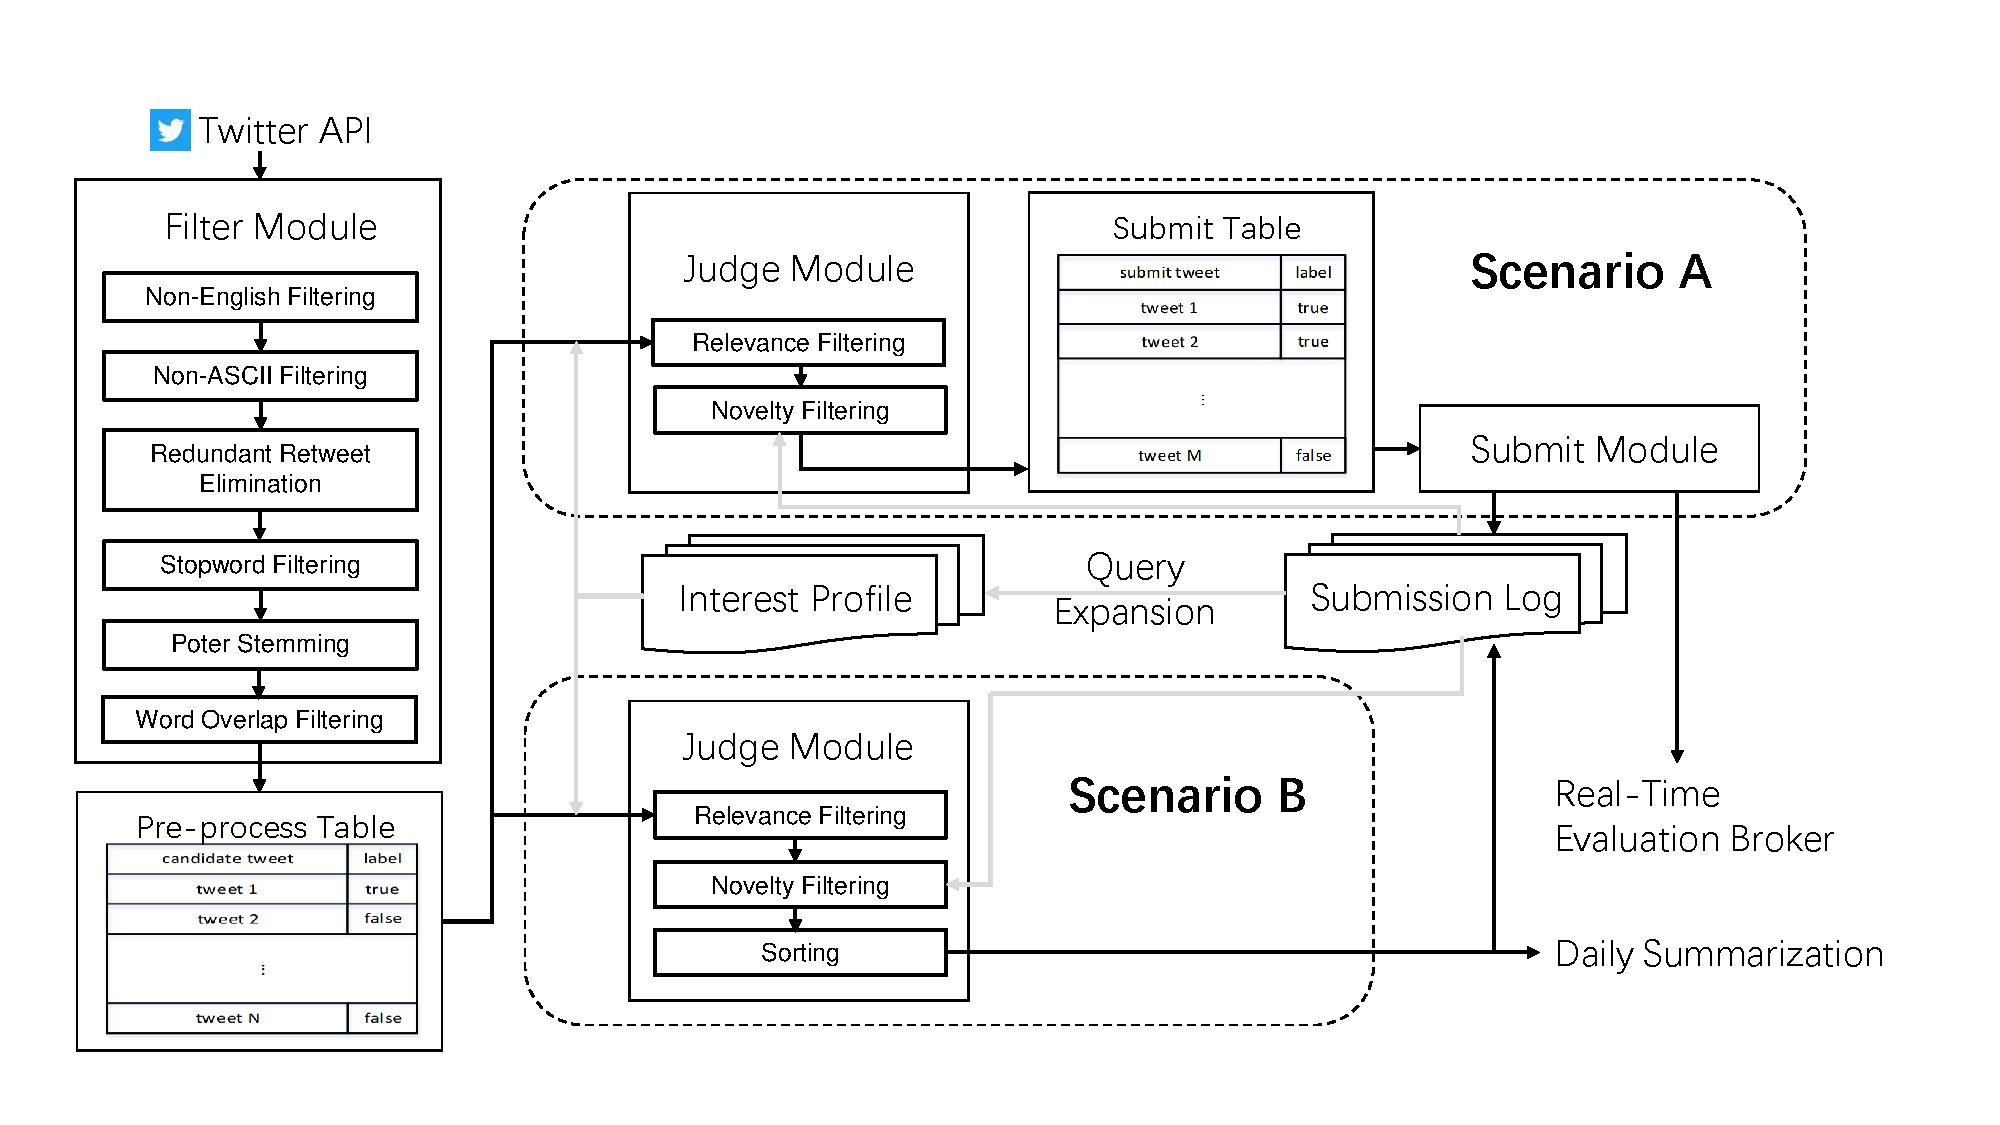
\epsfig{file=figures/system.pdf, width=\textwidth}
}
\caption{The System Architecture.}
\label{fig:system}
\end{figure*}

\subsection{Preliminaries}
In this section, we mainly talk about how our system perform preliminary operation,
to make the follow-up filtering easier and more precise.

\subsubsection{Filter Module}
The preprocessing we adopt on interest profile and tweet stream follows \cite{yao2016pkuicst} and \cite{lvpkuicst},
which is described as follows:

\begin{itemize}
\item \textbf{Non-English Filtering:}
Tweets written in a language other than English would be judged as not relevant
based on guidelines of Real-Time Summarization Track.
Thus, we use the twitter's language detector to abandon the non-English tweets.
\item \textbf{Non-ASCII Words:}
Removing all NON-ASCII characters from the tweets will also helps remove non-English tweets.
\item \textbf{Redundant Retweet Elimination:}
All additional commentary in the tweets containing ``RT @'' will be ignored.
As the guideline mentioned, all retweets should be normalized to the underlying tweets.
\item \textbf{Porter Stemming and Stopword Filtering:}
We remove all stopwords and stem the tweet text using the Natural Language Toolkit.
\item \textbf{Word Overlap Filtering:}
We filter out tweets that have no overlap with all interest profile in word-level,
because our methods don't consider semantic information. 
This can accelerate the he speed of identifying possible relevant tweets for each profile.
\end{itemize}

\subsubsection{Statistics Information}
In the language model, if any word in the query is not in the document,
the relevant score between them will equal to zero, which is unreasonable.
Smooth techniques could solve this problem by merging global word
probability distribution with current document model.
In our proposed approach, we obtain the global word probability distribution
by computing word count information of tweet stream during the 10 days before the evaluation period.

\subsection{Scenario A}
In this section, we will introduce our method for Scenario A.

\begin{itemize}
\item \textbf{Judge Module}
This module keeps 'listening' to the Pre-process Table. 
Every time a new inserted tweet is detected
(actually we collect a bunch of tweets in every time interval T1 in practice), 
that tweet is sent to the next stage for filtering. 
In the first stage of filtering, for every interest profile, we compute a relevance score 
using a text similarity function $f$. 
If that relevance score is bigger than the relevance threshold $\alpha$, 
this tweet-profile pair can go to the next stage.
In the second stage of filtering, for every selected tweet-profile pair, 
The same as previous stage, 
we compute the similarities using $f$ between the tweet and each of the pushed tweets of this profile,
we select the biggest one as the novelty score and compared to the novelty threshold $\beta$.
If that novelty score is smaller than $\beta$, 
we insert this tweet to the Submit Table, and remove it from the Pre-process Table.  
\item \textbf{Submit Module}
Like the Judge Module, this module keeps 'listening' to the Submit Table.
Every time a new inserted tweet is detected
(actually we collect a bunch of tweets in every time interval T2 in practice), 
that tweet is sent to the Evaluation Broker. 
If the response tell us the submission is accepted successfully,
we remove that tweet from the Submit Table and write it into the Submission Log.
Otherwise that tweet will stay in the Submit Table until a successful submission. 
\end{itemize} 


\subsubsection{Similarity Algorithm}

The key components of the Judge Module is the similarity function $f$.
We use $f$ to compute the similarity of (tweet, profile) pairs and (tweet, tweet) pairs.
Note that we only use the 'title' of each interest profile for computing similarities.
 
We utilize two different methods to model similarity.

\begin{itemize}
\item \textbf{negative KL-divergence language model}
One of the most powerful approach is language model. 
Each tweet $D$ and each interest profile $Q$ can be regard as a probability distribution.
We use notation $\widehat{\theta}_D$ and $\widehat{\theta}_Q$ to represent the language model respectively.
The negative KL-divergence between $\widehat{\theta}_Q$ and $\widehat{\theta}_D$ with the help of
collection language model $\widehat{\theta}_C$ can be calculated as below:

\begin{equation}
\begin{aligned}
DIR(Q,&D,C) = \sum_{w \in Q} P(w|\widehat{\theta}_Q) \cdot \\
&log \left( (1-\lambda) * P(w|\widehat{\theta}_D) + \lambda * P(w|\widehat{\theta}_C) \right), \\
with\; \lambda &= \frac{\mu}{|D| + \mu}
\end{aligned}
\end{equation}

\item \textbf{cosine distance}
Another method is using cosine distance model the similarity directly.
We build the IDF(Inverse Document Frequency) vector for each tweet and interest profile.
The IDF of each word is computed by the tweets collected before evaluation period,
as we have talked in the Preliminaries section.
The formula is shown below:

\begin{equation}
COS(Q,D) = \frac{\vec{Q} \cdot \vec{D}}{|\vec{Q}||\vec{D}|}
\end{equation}

\end{itemize}

\subsubsection{Query Expansion}

As microblog retrieval suffers severely from the vocabulary mismatch problem 
(i.e. term overlap between query and tweet is relatively small).
Query Expansion \cite{zhai2011mbfb} can play an important role in this situation. 
Moreover, more terms in the query makes retrieval more precise in general.

We use Pseudo Relevance Feedback technique to expand the interest profile 
with IDF-cosine method in PKUICSTRunA3 and PKUICSTRunB3.
At the end of each day, we collect the submitted tweets of each interest profile,
compute the word count, and sort by the word count.
For each interest profile, we add the top $K$ words that are not original in the profile to the profile.
We set the expanded words a weight $\gamma (\gamma < 1)$ while the original words with a default weight 1.  

\subsubsection{Parameter Selection}

The parameters shown in Table.\ref{tab:paraA} are tuned via grid search on TREC 2016 dataset.

\begin{table}[htbp]
\newcommand{\tabincell}[2]{\begin{tabular}{@{}#1@{}}#2\end{tabular}}
\centering
\caption{Parameters of the Push Notifications Scenario.}
\label{tab:paraA}
\begin{tabular}{lcccc}
\hline
Run ID&$f$&$\alpha$&$\beta$&\tabincell{c}{Query\\Expansion}\\
\hline
PKUICSTRunA1&\tabincell{c}{DIR\\$\mu=50$}&0.7&0.5&-\\
PKUICSTRunA2&COS&0.8&0.85&-\\
PKUICSTRunA3&COS&0.8&0.85&\tabincell{c}{$K=2$\\$\gamma=0.2$}\\
\hline
\end{tabular}
\end{table}

\subsection{Scenario B}

From Figure.\ref{fig:system}, we can see our approach of Scenario B is not much different from that of Scenario A.
We remove the Submit Module and Submit Table, and add a sorting process at the end of Judge Module.
Besides, we try to utilize model blending in this scenario.
Model blending has been proved useful in many situation.
We simply use the formula below to blend our two similarity models discussed before.

\begin{equation}
\begin{aligned}
BL(Q,D,C) = &\delta \cdot DIR(Q,D,C)+ \\
&(1-\delta)\cdot COS(Q,D), 0 < \delta < 1
\end{aligned}
\end{equation}   

\subsubsection{Parameter Selection}

Like Scenario A, these parameters shown in Table.\ref{tab:paraB} are tuned via grid search on TREC 2016 dataset.

\begin{table}[htbp]
\newcommand{\tabincell}[2]{\begin{tabular}{@{}#1@{}}#2\end{tabular}}
\centering
\caption{Parameters of the Push Notifications Scenario.}
\label{tab:paraB}
\begin{tabular}{lcccc}
\hline
Run ID&$f$&$\alpha$&$\beta$&\tabincell{c}{Query\\Expansion}\\
\hline
PKUICSTRunB1&\tabincell{c}{DIR\\$\mu=50$}&0.72&0.72&-\\
PKUICSTRunB2&\tabincell{c}{BL\\$\mu=50$ \\ $\delta=0.5$ }&0.78&0.78&-\\
PKUICSTRunB3&\tabincell{c}{BL\\$\mu=50$ \\ $\delta=0.5$}&0.78&0.78&\tabincell{c}{$K=2$\\$\gamma=0.2$}\\
\hline
\end{tabular}
\end{table}

\section{Experiment}
The evaluation of TREC 2017 Real-time Summarization track takes place from
July 25, 2017 UTC to August 3, 2017 UTC.

\subsection{Scenario A}
For Scenario A, there are two main assessment approaches.

One is Mobile Assessment. Mobile assessors receive pushed tweets immediately, 
and judge whether that tweet is relevant, redundant or non-relevant.
The strict precision is the proportion of relevant tweets pushed by a run,
and the lenient precision is the proportion of relevant and redundant tweets pushed by a run.
This time, assessors judged 188 topics(with uneven effort), 
and the results of Mobile Assessment are shown in Table.\ref{tab:A_mobile}.

Another assessment approach is NIST Assessment. 
This assessment has multiple metrics, 
including Expected Gain (EG) and Normalized Cumulative Gain (nCG).
There two variants of EG, EG-1 and EG-p.
In EG-1 metrics, on a silent day,  
the system receives a score of one (i.e., perfect score) if it does not push any tweets.
While in EG-p, on a silent day, 
the score is one minus the fraction of the ten-tweet daily quota that is used. 
Similarly, we can define nCG-1 and nCG-p.
The results of NIST Assessment are shown in Table.\ref{tab:A_NIST}

We can observe that different approaches of modelling similarity have different preferences.
In PKUICSTRunA2 and PKUICSTRunA3, we select IDF-cosine algorithm and a relative high relevance threshold.
That makes PKUICSTRunA2 and PKUICSTRunA3 get higher score in precision.
But higher threshold also means the system tends not to push the tweets, 
witch makes these systems perform bad in some macro-averaged metrics
(because it's common for these systems to push nothing all day), like EG and nCG.
Additionally, from the comparison of PKUICSTRunA2 and PKUICSTRunA3, 
we learn that a good query expansion method really helps a lot,
and pseudo relevance feedback technique can be a choice.     

\begin{table}[htbp]
\centering
\caption{Scenario A Mobile Assessment.}
\label{tab:A_mobile}
\begin{tabular}{lrr}
\hline
Run ID&strict precision&lenient precision\\
\hline
PKUICSTRunA1&0.3108&0.3642\\
PKUICSTRunA2&0.3673&0.4174\\
PKUICSTRunA3&\textbf{0.3863}&\textbf{0.4340}\\
\hline
\end{tabular}
\end{table}

\begin{table}[htbp]
\centering
\caption{Scenario A NIST Assessment.}
\label{tab:A_NIST}
\begin{tabular}{lrrrr}
\hline
Run ID&EGp&EG1&nCGp&nCG1\\
\hline
PKUICSTRunA1&\textbf{0.2869}&\textbf{0.2588}&\textbf{0.2864}&\textbf{0.2583}\\
PKUICSTRunA2&0.1959&0.1866&0.1866&0.1774\\
PKUICSTRunA3&0.1997&0.1892&0.1908&0.1804\\
\hline
\end{tabular}
\end{table}

\subsection{Scenario B}

Table.\ref{tab:B_NIST} reports our results for the email digest scenario.
The main evaluation metric is nDCG-p and nDCG-1.

As we keep our parameter setting in Senario B similar to that in Senario A,
the performance of our system in Scenario B have the same trend with that in Scenario A. 
It shows that our two-stage filtering approach also perform well in a non-real-time task.

\begin{table}[htbp]
\centering
\caption{Scenario B NIST Assessment.}
\label{tab:B_NIST}
\begin{tabular}{lrr}
\hline
Run ID&nDCGp&nDCG1\\
\hline
PKUICSTRunB1&\textbf{0.3483}&\textbf{0.3003}\\
PKUICSTRunB2&0.1968&0.1809\\
PKUICSTRunB3&0.2306&0.2024\\
\hline
\end{tabular}
\end{table}



\section{Conclusion}
In this paper, we present our systems for TREC 2017 Real-Time Summarization Track.
We design a two-stage filtering system for both Scenario A and B, 
and utilize two kinds of text similarity model, 
language model with negative KL-divergence and IDF with cosine distance.
Pseudo relevance feedback technique is tried to do query expansion.
Particularly, a decoupled real-time system are designed for Scenario A.
Experimental results show our effectiveness and efficiency of our system in both tasks.




\section{Acknowledgments}
The work reported in this paper is supported by the National Natural Science Foundation of China Grant 61370116.

\bibliographystyle{aaai}
\bibliography{yelp}
\end{document}
